% gougu.tex
% 勾股定理
 
\documentclass[UTF8]{ctexart}
\usepackage{graphicx}	% 插入图所需宏包
\usepackage{float}	% float 宏包为 figure 环境加上了一个 [H]  位置选项,从而使得用 figure 环境可以生成不浮动的图形。
\usepackage{amsmath}	% 公式的交叉引用
\usepackage{geometry}
 
\geometry{a6paper,centering,scale=0.8}
\usepackage[format=hang,font=small,textfont=it]{caption}	% 设定图表所有标题使用悬挂对齐方式(即编号向左突出),整体用小字号,而标题文本使用斜体(对汉字来说就是楷书)。
 
\usepackage[nottoc]{tocbibind}	% 宏包默认会在目录中加入目录项本身、参考文献、索引等项目。这里使用 nottoc 选项取消了在项目中显示目录本身。
\usepackage{syntonly}
 
\title{\heiti 杂谈勾股定理}
\author{\kaishu 张三}
\date{\today}
 
\newtheorem{thm}{定理}
\bibliographystyle{unsrt}
%\bibliographystyle{plain}
 
\newenvironment{myquote}{\begin{quote}\zihao{-5}\kaishu}{\end{quote}}	% 引用部分格式定义
 
\newcommand\degree{^\circ}
 
% 之前都是导言区
 
\begin{document}
 
	\maketitle
	
	\begin{abstract}
		这是一篇勾股定理的小短文。
	\end{abstract}
 
	\tableofcontents
 
	\section{勾股定理在古代}\label{sec:first}
	西方称勾股定理为毕达哥拉斯定理,将勾股定理的发现归功于公元前 6 世纪的毕达哥拉斯学派 \cite{kline}。该学派得到了一个法则,可以求出可排成直角三角形三边的三元数组。毕达哥拉斯学派没有书面著作,该定理的严格表述和证明则见于欧几里得\footnote{欧几里得,约公元前 330-275 年。}《几何原本》的命题 47:“直角三角形斜边上的正方向形等于两直角边上的两个正方形之和。”证明是用面积做的。
	
	我国《周脾算经》载商高(约公元前 12 世纪)答周公问:
	\begin{myquote}
		勾广三,股修四,径隅五。
	\end{myquote}
	又载陈子(约公元前 7--6 世纪)答荣方问:
	\begin{myquote} 
		若求邪至日者,以日下为勾,日高为股,勾股各自乘,并而开方除之,得邪至日。
	\end{myquote}
	都比古希腊更早。后者已经明确道出勾股定理的一般形式。图\ref{fig:xiantu}是我国古代对勾股定理的一种证明 \cite{quanjing}。
	\begin{figure}[ht] 
		\centering
		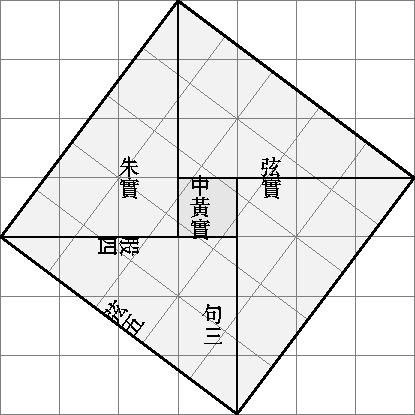
\includegraphics[scale=0.2]{xiantu.pdf}
		\caption{宋赵爽在《周脾算经》注中作的弦图(仿制),该图给出了勾股定理的一个极具对称美的证明。}
		\label{fig:xiantu}
	\end{figure}
	
	
	\section{勾股定理的近代形式}
	勾股定理可以用现代语言表述如下:
	\begin{thm}[勾股定理]
		直角三角形斜边的平方等于两腰的平方和。
		
		可以用符号语言表述为:设直角三角形$ABC$,其中$\angle C=90\degree$,则有
		\begin{equation}\label{eq:gougu}
			AB^2 = BC^2 + AC^2.
		\end{equation}
	\end{thm}
 
	满足式\eqref{eq:gougu}的整数称为\emph{勾股数}。第\ref{sec:first}节所说毕达哥拉斯学派得到的三元数组就是勾股数。下表列出了一些较小的勾股数:
	\begin{table}[H]
		\begin{tabular}{|rrr|}
			\hline
			直角边 $a$ & 直角边 $b$ & 斜边 $c$ \\
			\hline
			3    & 4    & 5   \\
			5    & 12   & 13 \\
			\hline
		\end{tabular}%
	\qquad
	($a^2 + b^2 = c^2$)
	\end{table}
 
	\nocite{Shiye}
	\bibliography{math}
\end{document}
